\documentclass[12pt,a4paper]{article}

\usepackage[top=1in,bottom=1in,left=1.25in,right=1in]{geometry}
\renewcommand{\rmdefault}{ptm}
\usepackage{setspace}
\usepackage{graphicx}
\usepackage{tabularx}
\usepackage{booktabs}
\usepackage{array}
\usepackage{float}
\usepackage{caption}
\usepackage{hyperref}
\usepackage{tikz}
\usetikzlibrary{arrows.meta,positioning,shapes.geometric,fit,calc}
\usepackage{xcolor}
\usepackage{fancyhdr}
\usepackage{titlesec}

\onehalfspacing
\setlength{\parindent}{0pt}
\setlength{\parskip}{6pt}

\titleformat{\section}
  {\normalfont\fontsize{16}{19}\bfseries}{\thesection}{1em}{}
\titleformat{\subsection}
  {\normalfont\fontsize{14}{17}\bfseries}{\thesubsection}{1em}{}
\titleformat{\subsubsection}
  {\normalfont\fontsize{12}{15}\bfseries}{\thesubsubsection}{1em}{}

\captionsetup{font=bf,labelfont=bf}
\renewcommand{\contentsname}{Contents}

\pagestyle{fancy}
\fancyhf{}
\fancyfoot[C]{\thepage}
\renewcommand{\headrulewidth}{0pt}
\fancypagestyle{plain}{\fancyhf{}\fancyfoot[C]{\thepage}\renewcommand{\headrulewidth}{0pt}}

\hypersetup{
  colorlinks=true,
  linkcolor=black,
  citecolor=black,
  urlcolor=blue
}

\begin{document}

\hypersetup{pageanchor=false}
\begin{titlepage}
\begin{center}

\textbf{\fontsize{14}{17}\selectfont Lincoln University College}\\[4pt]
\textbf{\fontsize{12}{15}\selectfont Faculty of Computer Science and Multimedia}\\[28pt]

\textbf{\fontsize{16}{19}\selectfont PocketDRS: A Single-View 3D Trajectory\\
Reconstruction and Decision Review System for Cricket}\\[24pt]

\textbf{\fontsize{14}{17}\selectfont MID DEFENSE REPORT}\\[10pt]
\fontsize{12}{15}\selectfont
Submitted to\\[4pt]
Department of Information Technology\\
Phoenix College of Management\\
Maitidevi, Kathmandu\\[20pt]

In partial fulfillment of the requirements for the degree of\\
\textbf{Bachelor in Information Technology (BIT)}\\[24pt]

Submitted by\\[8pt]
\textbf{Niraj Kafle}\\
BIT 7th Semester\\
University ID: LC0003001674\\[30pt]

\vfill
\textbf{March, 2026}

\end{center}
\end{titlepage}

\clearpage
\hypersetup{pageanchor=true}
\pagenumbering{roman}
\tableofcontents

\clearpage
\pagenumbering{arabic}

\section{Introduction}

Cricket officiating increasingly depends on technology for reviewing close decisions, especially Leg Before Wicket (LBW) cases. In elite matches, systems such as Hawk-Eye reconstruct the ball trajectory using multiple synchronized high-speed cameras and specialized processing infrastructure. Although these systems are highly effective, they are costly, complex to operate, and impractical for schools, clubs, local leagues, and training environments \cite{hawkeye2024}.

PocketDRS is proposed as a low-cost decision-support system that uses a single smartphone camera and a lightweight backend service to analyze a delivery. The user records or selects a short video clip, calibrates the visible pitch by marking known reference points, submits the delivery for processing, and receives a visual explanation together with an LBW assessment.

The project emphasizes practicality over broadcast-grade precision. The goal is not to replace certified professional DRS, but to demonstrate that a constrained single-view pipeline can provide meaningful review support in low-resource cricket settings. The current prototype focuses on reliable pitch-plane tracking, event detection, and explainable visualization, while acknowledging the accuracy limits of monocular analysis.

\section{Problem Statement}

Professional DRS systems depend on multiple synchronized cameras to recover depth and reconstruct the trajectory of the ball in three dimensions. This produces strong results, but the required equipment, installation effort, and operating cost make such systems inaccessible outside major venues.

When the same decision-review problem is shifted to a single consumer camera, several technical and practical difficulties arise:

\begin{enumerate}
    \item A monocular view does not provide direct depth information.
    \item A cricket ball is small, fast, motion-blurred, and can easily be confused with background objects.
    \item Small calibration errors can produce large errors when detections are mapped to pitch coordinates.
    \item Lighting variation, camera shake, player occlusion, and inconsistent recording conditions reduce reliability in real grounds.
\end{enumerate}

Therefore, the central problem addressed by this project is whether a single-phone-camera workflow, supported by pitch calibration and lightweight computer-vision techniques, can produce a sufficiently consistent and understandable LBW review aid for ordinary cricket grounds.

\section{Objectives}

\subsection{General Objective}

To design and implement a low-cost cricket decision-support system that uses a single camera view to analyze a delivery, estimate the ball path in calibrated pitch coordinates, and assist LBW review.

\subsection{Specific Objectives}

\begin{enumerate}
    \item Study existing decision-review systems and relevant literature on monocular sports tracking.
    \item Develop a user-guided calibration process based on pitch corners and stump reference points.
    \item Detect and track the ball from delivery video using combined motion and colour cues.
    \item Map tracked pixel positions to pitch-plane coordinates using homography.
    \item Detect important events such as bounce and impact from the tracked trajectory.
    \item Estimate an LBW outcome using rule-based checks on pitching line, impact line, and projected stump contact.
    \item Present the result through a simple interactive visualization that helps users interpret the decision.
\end{enumerate}

\section{Methodology}

\subsection{Requirement Identification}

\subsubsection{Study of Existing System}

Existing systems such as Hawk-Eye use multiple calibrated cameras, controlled camera placement, high frame rates, and proprietary reconstruction pipelines. These systems are designed for professional broadcasting environments. In contrast, PocketDRS adopts a constrained workflow built for affordability: one mobile camera, one short trimmed delivery clip, one user-guided calibration step, and a lightweight server-side analysis pipeline. The trade-off is lower accuracy than professional systems, but much lower deployment cost and complexity.

\subsubsection{Literature Review}

Related research shows that single-view sports analysis becomes more feasible when the scene contains known geometry and the target motion follows domain constraints. In cricket, the pitch provides stable reference landmarks, while the ball generally follows a predictable sequence from release to bounce, then impact, and finally the projected wicket line. Homography-based mapping from image coordinates to a known plane is a practical way to convert 2D observations into real-world pitch coordinates \cite{zhang2000}. Background subtraction and colour filtering remain effective low-cost detection strategies in controlled or semi-controlled environments, especially when the search space is reduced through domain knowledge \cite{opencv2024}. Recent work on monocular ball trajectory estimation further suggests that strong constraints can compensate for missing depth information, although monocular systems remain more fragile than multi-camera solutions \cite{ponglertnapakorn2021}. These findings support the feasibility of a student-scale prototype that prioritizes explainability and affordability.

\subsubsection{Requirement Analysis}

\textbf{Functional requirements}

\begin{enumerate}
    \item User signs in.
    \item User records or selects a video.
    \item User creates or reuses pitch calibration.
    \item User trims the clip and submits it.
    \item Server tracks the ball through the selected segment.
    \item Server maps the track to pitch coordinates.
    \item Server detects bounce and impact points.
    \item Server evaluates the LBW outcome.
    \item App shows the decision, warnings, and an interactive visual result.
\end{enumerate}

\textbf{Non-functional requirements}

\begin{enumerate}
    \item The system should stay easy to use for a first-time user.
    \item Processing should finish in a short time for one delivery.
    \item The app should run on both Android and iOS.
    \item The server should work with common phone video quality and practical frame rates.
    \item The final result should be understandable to non-technical users.
    \item The system should provide diagnostic warnings when calibration or tracking quality is weak.
    \item The architecture should remain modular so that stronger tracking or reconstruction methods can be added later.
\end{enumerate}

\begin{figure}[htbp]
\centering
\resizebox{0.96\textwidth}{!}{%
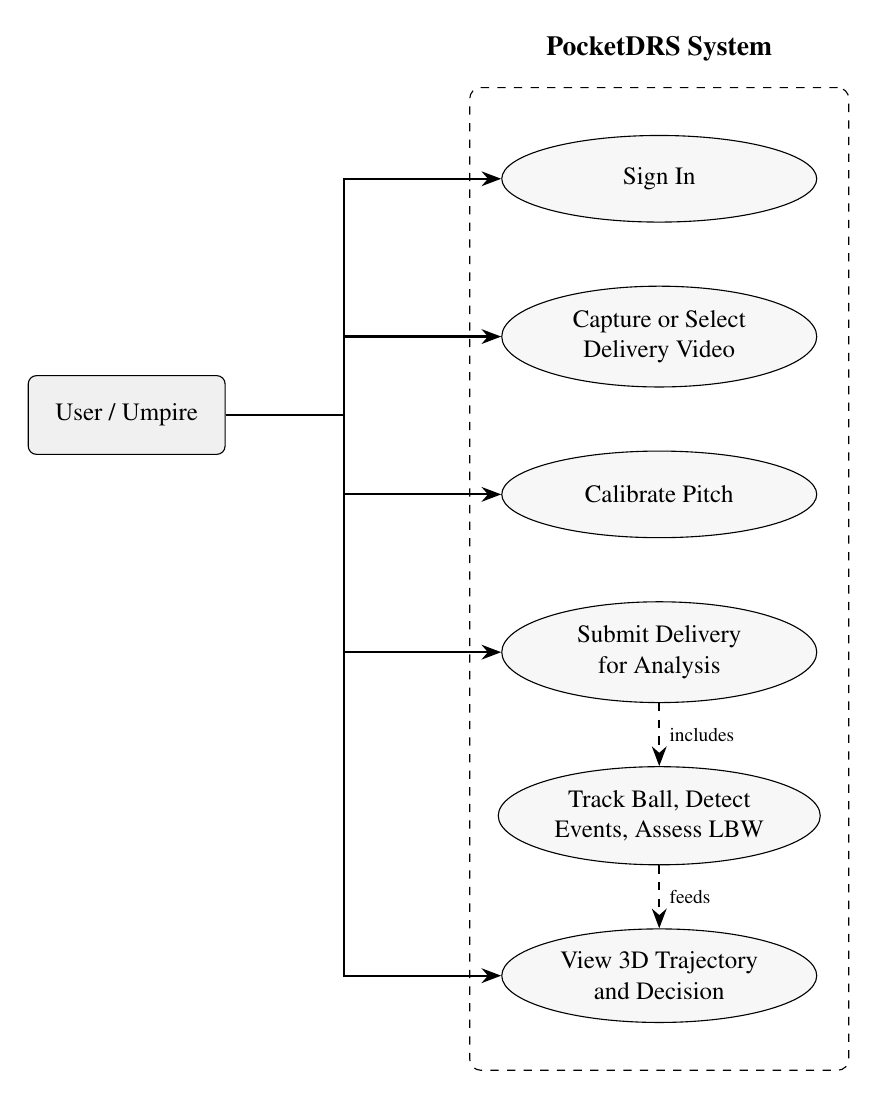
\begin{tikzpicture}[
    node distance=1.0cm and 2.5cm,
    entity/.style={draw, rounded corners=3pt, minimum width=2.5cm, minimum height=1cm, align=center, font=\small, fill=gray!12},
    usecase/.style={draw, ellipse, minimum width=4cm, minimum height=1.1cm, align=center, font=\small, fill=gray!6},
    sys/.style={draw, dashed, rounded corners=4pt, inner xsep=0.4cm, inner ysep=0.6cm},
    rel/.style={-{Stealth[length=2.5mm]}, line width=0.8pt},
    note/.style={font=\scriptsize, align=center}
]

\node[entity] (user) {User / Umpire};

\node[usecase, right=3.5cm of user, yshift=3.0cm] (u1) {Sign In};
\node[usecase, below=0.8cm of u1] (u2) {Capture or Select\\Delivery Video};
\node[usecase, below=0.8cm of u2] (u3) {Calibrate Pitch};
\node[usecase, below=0.8cm of u3] (u4) {Submit Delivery\\for Analysis};
\node[usecase, below=0.8cm of u4] (u5) {Track Ball, Detect\\Events, Assess LBW};
\node[usecase, below=0.8cm of u5] (u6) {View 3D Trajectory\\and Decision};

\node[sys, fit=(u1)(u6), label={[font=\bfseries, yshift=2mm]above:PocketDRS System}] (sysbox) {};

\draw[rel] (user.east) -- ++(1.5,0) |- (u1.west);
\draw[rel] (user.east) -- ++(1.5,0) |- (u2.west);
\draw[rel] (user.east) -- ++(1.5,0) |- (u3.west);
\draw[rel] (user.east) -- ++(1.5,0) |- (u4.west);
\draw[rel] (user.east) -- ++(1.5,0) |- (u6.west);

\draw[dashed, rel] (u4.south) -- node[note, right] {includes} (u5.north);
\draw[dashed, rel] (u5.south) -- node[note, right] {feeds} (u6.north);
\end{tikzpicture}
}
\caption{Main use cases of PocketDRS.}
\label{fig:usecase}
\end{figure}

\subsection{Feasibility Study}

\subsubsection{Technical Feasibility}

The proposed system is technically feasible because it is built from mature and widely supported technologies. Flutter provides cross-platform mobile development, FastAPI provides lightweight and testable backend services, OpenCV supports frame processing and tracking, and Firebase handles authentication and cloud persistence. The present implementation already demonstrates upload, calibration, server-side analysis, and result visualization on consumer devices. Although monocular video imposes accuracy limits, the required software stack is realistic for a student project and deployable on ordinary hardware.

\subsubsection{Operational Feasibility}

The operational workflow is simple enough for field use during testing and demonstrations. A user places a phone near square leg or a side-on view, records a delivery, calibrates the pitch by tapping known points, trims the clip, and waits for the generated result. This procedure is repeatable, requires minimal training, and fits the needs of clubs, student projects, and coaching sessions.

\subsubsection{Economic Feasibility}

The project is economically feasible because it does not require specialized camera arrays, licensed broadcast systems, or custom hardware. It relies primarily on a smartphone, a tripod, and open-source libraries. Compared with professional DRS infrastructure, the expected deployment cost is extremely low, making the proposed system suitable for academic demonstration and low-budget cricket environments.

\begin{table}[htbp]
\centering
\caption{Main tools used in PocketDRS.}
\label{tab:stack}
\begin{tabularx}{\textwidth}{@{}lX@{}}
\toprule
\textbf{Part} & \textbf{Tool} \\
\midrule
Mobile app & Flutter and Dart \\
Server API & FastAPI and Python \\
Vision pipeline & OpenCV, NumPy, SciPy \\
Authentication & Firebase Authentication \\
Data storage & Cloud Firestore \\
3D result view & Three.js inside WebView \\
Testing & pytest and Flutter analyzer \\
\bottomrule
\end{tabularx}
\end{table}

\subsection{High Level Design of System}

The proposed system is designed as a mobile-to-server workflow. The mobile application handles video capture or selection, pitch calibration, job submission, and result presentation. The backend decodes the selected segment, tracks the ball, computes a homography from user-provided pitch points, maps detections to pitch coordinates, detects key events, evaluates the LBW decision, and returns structured output to the client. The following diagrams summarize the architecture, data flow, software components, deployment structure, and working mechanism of the system.

\begin{figure}[htbp]
\centering
\resizebox{0.6\textwidth}{!}{%
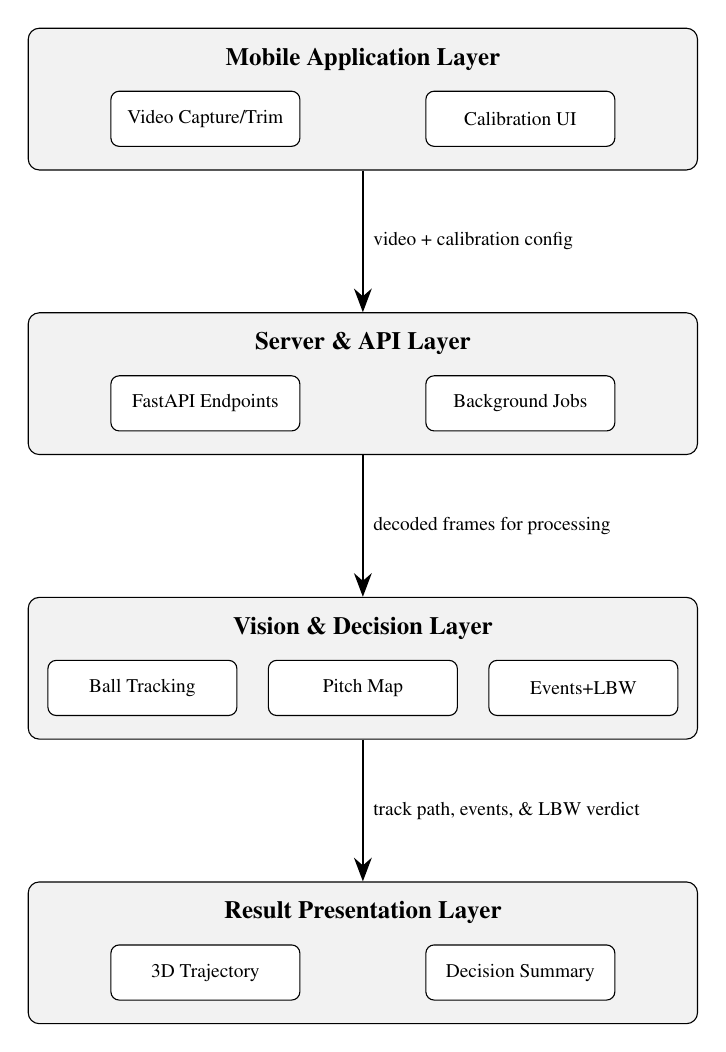
\begin{tikzpicture}[
    node distance=1.5cm,
    layer/.style={draw, rounded corners=4pt, minimum width=8.5cm, minimum height=1.8cm, align=center, font=\small, fill=gray!10},
    smallbox/.style={draw, rounded corners=3pt, minimum width=2.4cm, minimum height=0.7cm, align=center, font=\scriptsize, fill=white},
    flow/.style={-{Stealth[length=3mm]}, line width=0.9pt}
]

\node[layer] (mobile) {};
\node[font=\small\bfseries] at (mobile.north) [yshift=-4mm] {Mobile Application Layer};
\node[smallbox] (m1) at ([xshift=-2.0cm,yshift=-2.5mm]mobile.center) {Video Capture/Trim};
\node[smallbox] (m2) at ([xshift=2.0cm,yshift=-2.5mm]mobile.center) {Calibration UI};

\node[layer, below=1.8cm of mobile] (api) {};
\node[font=\small\bfseries] at (api.north) [yshift=-4mm] {Server \& API Layer};
\node[smallbox] (a1) at ([xshift=-2.0cm,yshift=-2.5mm]api.center) {FastAPI Endpoints};
\node[smallbox] (a2) at ([xshift=2.0cm,yshift=-2.5mm]api.center) {Background Jobs};

\node[layer, below=1.8cm of api] (pipeline) {};
\node[font=\small\bfseries] at (pipeline.north) [yshift=-4mm] {Vision \& Decision Layer};
\node[smallbox] (p1) at ([xshift=-2.8cm,yshift=-2.5mm]pipeline.center) {Ball Tracking};
\node[smallbox] (p2) at ([xshift=0,yshift=-2.5mm]pipeline.center) {Pitch Map};
\node[smallbox] (p3) at ([xshift=2.8cm,yshift=-2.5mm]pipeline.center) {Events+LBW};

\node[layer, below=1.8cm of pipeline] (result) {};
\node[font=\small\bfseries] at (result.north) [yshift=-4mm] {Result Presentation Layer};
\node[smallbox] (r1) at ([xshift=-2.0cm,yshift=-2.5mm]result.center) {3D Trajectory};
\node[smallbox] (r2) at ([xshift=2.0cm,yshift=-2.5mm]result.center) {Decision Summary};

\draw[flow] (mobile.south) -- node[right, font=\scriptsize, align=center] {video + calibration config} (api.north);
\draw[flow] (api.south) -- node[right, font=\scriptsize, align=center] {decoded frames for processing} (pipeline.north);
\draw[flow] (pipeline.south) -- node[right, font=\scriptsize, align=center] {track path, events, \& LBW verdict} (result.north);
\end{tikzpicture}
}
\caption{Overall architecture of PocketDRS.}
\label{fig:highlevel}
\end{figure}

\subsubsection{Context Level DFD}

\begin{figure}[htbp]
\centering
\resizebox{0.96\textwidth}{!}{%
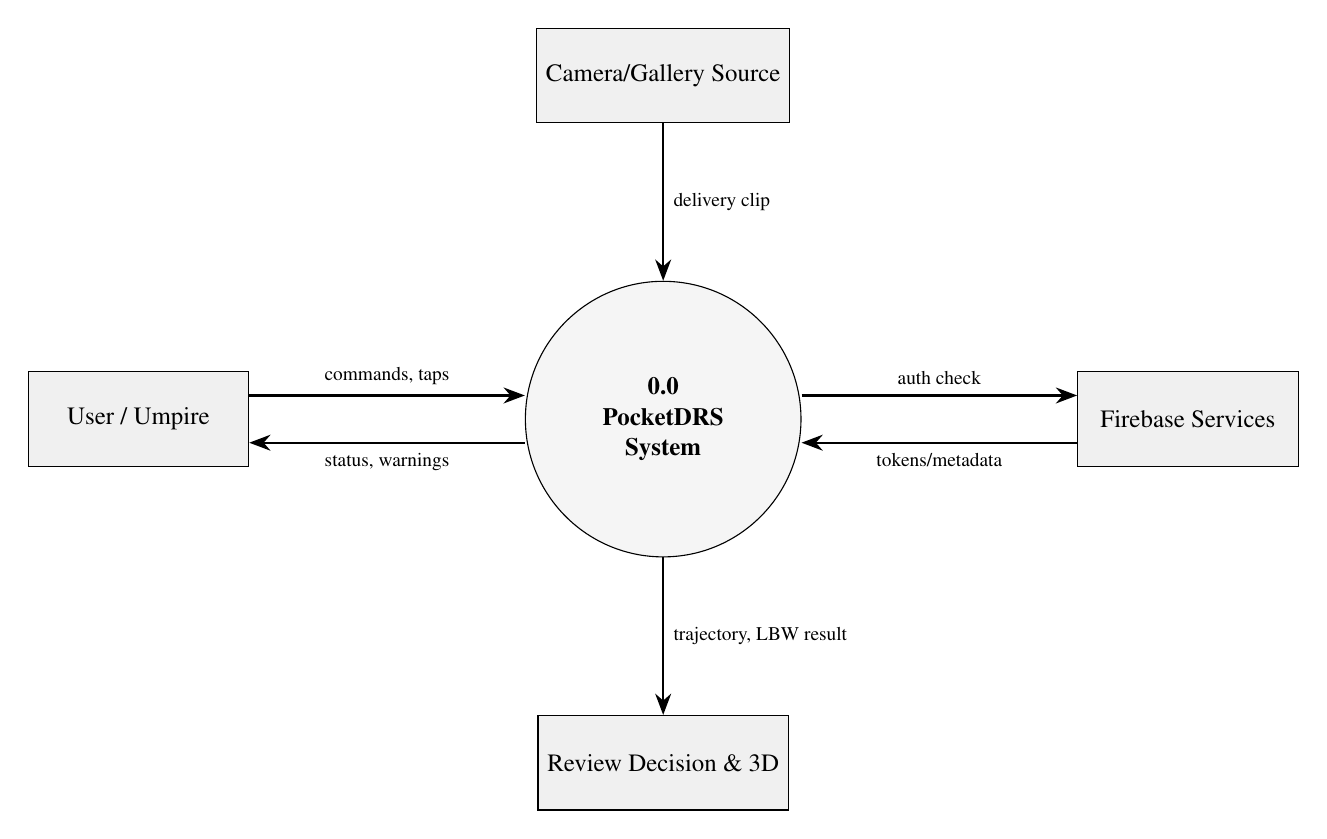
\begin{tikzpicture}[
    node distance=2.5cm and 3.5cm,
    ext/.style={draw, minimum width=2.8cm, minimum height=1.2cm, align=center, font=\small, fill=gray!12},
    proc/.style={draw, circle, minimum size=3.5cm, align=center, font=\small\bfseries, fill=gray!8},
    data/.style={-{Stealth[length=2.7mm]}, line width=0.8pt},
    lbl/.style={font=\scriptsize, align=center}
]

\node[proc] (system) {0.0\\PocketDRS\\System};
\node[ext, left=3.5cm of system] (user) {User / Umpire};
\node[ext, above=2cm of system] (media) {Camera/Gallery Source};
\node[ext, right=3.5cm of system] (firebase) {Firebase Services};
\node[ext, below=2cm of system] (result) {Review Decision \& 3D};

\draw[data, transform canvas={yshift=3mm}] (user.east) -- node[lbl, above] {commands, taps} (system.west);
\draw[data, transform canvas={yshift=-3mm}] (system.west) -- node[lbl, below] {status, warnings} (user.east);
\draw[data] (media.south) -- node[lbl, right] {delivery clip} (system.north);
\draw[data, transform canvas={yshift=3mm}] (system.east) -- node[lbl, above] {auth check} (firebase.west);
\draw[data, transform canvas={yshift=-3mm}] (firebase.west) -- node[lbl, below] {tokens/metadata} (system.east);
\draw[data] (system.south) -- node[lbl, right] {trajectory, LBW result} (result.north);
\end{tikzpicture}
}
\caption{Context-level DFD of PocketDRS.}
\label{fig:dfd-context}
\end{figure}

\subsubsection{Level 1 DFD}

\begin{figure}[htbp]
\centering
\resizebox{0.96\textwidth}{!}{%
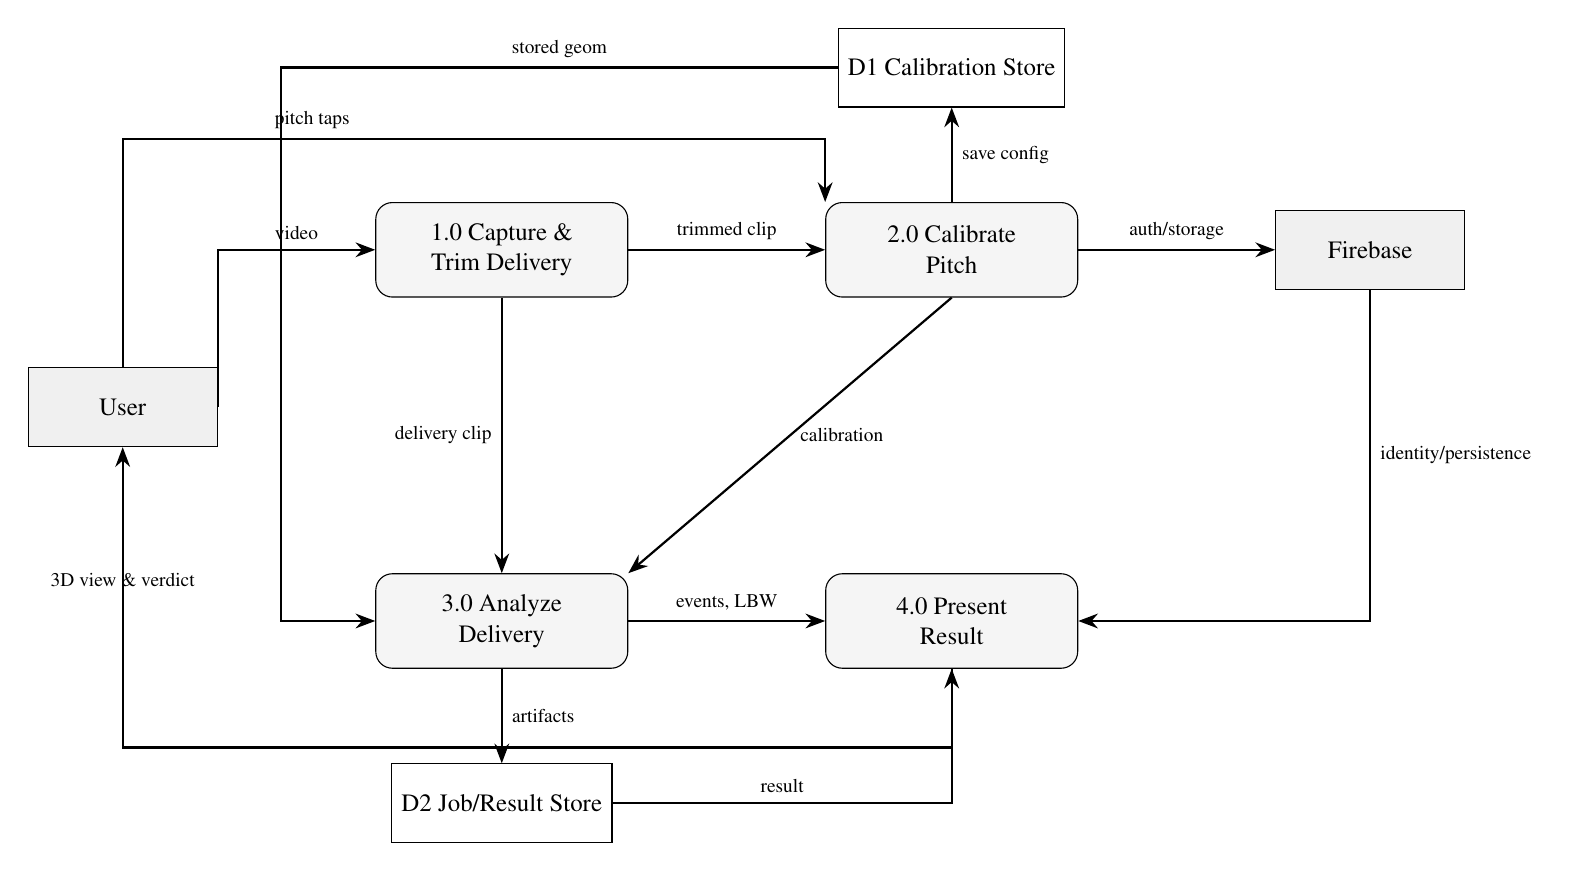
\begin{tikzpicture}[
    node distance=1.5cm and 2cm,
    ext/.style={draw, minimum width=2.4cm, minimum height=1cm, align=center, font=\small, fill=gray!12},
    proc/.style={draw, rounded corners=6pt, minimum width=3.2cm, minimum height=1.2cm, align=center, font=\small, fill=gray!8},
    store/.style={draw, minimum width=2.8cm, minimum height=1cm, align=center, font=\small, fill=white},
    flow/.style={-{Stealth[length=2.5mm]}, line width=0.8pt},
    lbl/.style={font=\scriptsize, align=center}
]

\node[ext] (user) {User};
\node[proc, right=2.0cm of user, yshift=2.0cm] (p1) {1.0 Capture \&\\Trim Delivery};
\node[proc, right=2.5cm of p1] (p2) {2.0 Calibrate\\Pitch};
\node[ext, right=2.5cm of p2] (firebase) {Firebase};

\node[proc, below=3.5cm of p1] (p3) {3.0 Analyze\\Delivery};
\node[proc, below=3.5cm of p2] (p4) {4.0 Present\\Result};

\node[store, above=1.2cm of p2] (d1) {D1 Calibration Store};
\node[store, below=1.2cm of p3] (d2) {D2 Job/Result Store};

\draw[flow] (user.east) |- node[lbl, above, pos=0.75] {video} (p1.west);
\draw[flow] (user.north) |- node[lbl, above, near end] {pitch taps} ([yshift=8mm]p1.north) -| (p2.north west);

\draw[flow] (p1.east) -- node[lbl, above] {trimmed clip} (p2.west);
\draw[flow] (p2.north) -- node[lbl, right] {save config} (d1.south);
\draw[flow] (p2.south) -- node[lbl, right] {calibration} (p3.north east);
\draw[flow] (p1.south) -- node[lbl, left] {delivery clip} (p3.north);

\draw[flow] (d1.west) -| node[lbl, near start, above] {stored geom} ([xshift=-1.2cm]p1.west) |- (p3.west);

\draw[flow] (p3.east) -- node[lbl, above] {events, LBW} (p4.west);
\draw[flow] (p3.south) -- node[lbl, right] {artifacts} (d2.north);
\draw[flow] (d2.east) -| node[lbl, near start, above] {result} (p4.south);

\draw[flow] (p2.east) -- node[lbl, above] {auth/storage} (firebase.west);
\draw[flow] (firebase.south) |- node[lbl, right, near start] {identity/persistence} (p4.east);

\draw[flow] (p4.south) |- ++(0,-1cm) -| node[lbl, above, near end] {3D view \& verdict} (user.south);
\end{tikzpicture}
}
\caption{Level-1 DFD of the PocketDRS processing workflow.}
\label{fig:dfd-level1}
\end{figure}

\subsubsection{Working Flow}

The working flow is kept short so that users can perform the analysis with minimal overhead:

\begin{figure}[htbp]
\centering
\resizebox{0.96\textwidth}{!}{%
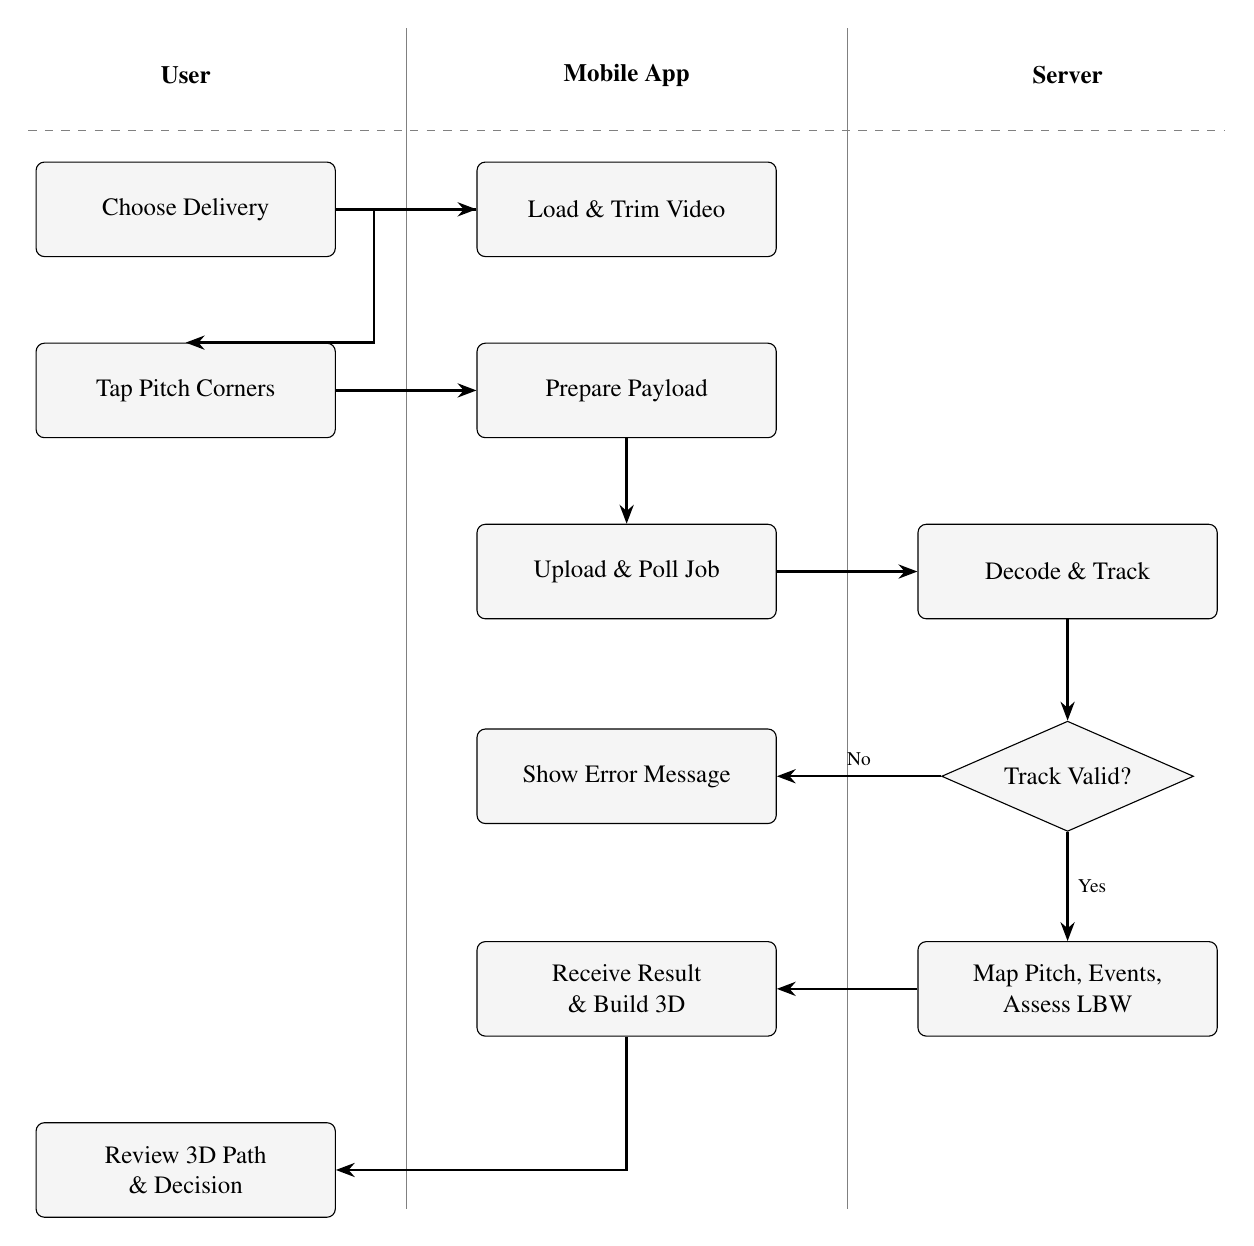
\begin{tikzpicture}[
    head/.style={font=\small\bfseries, align=center},
    flowstep/.style={draw, rounded corners=3pt, minimum width=3.8cm, minimum height=1.2cm, align=center, font=\small, fill=gray!8},
    decision/.style={draw, diamond, aspect=2.1, minimum width=3.2cm, minimum height=1.4cm, align=center, font=\small, fill=gray!8},
    arrow/.style={-{Stealth[length=2.4mm]}, line width=0.85pt}
]

\def\w{5.6}
\node[head] (h1) at (-\w, 0) {User};
\node[head] (h2) at (0, 0) {Mobile App};
\node[head] (h3) at (\w, 0) {Server};

\draw[dashed, gray] (-\w-2.0, -0.7) -- (\w+2.0, -0.7);
\draw[gray] (-0.5*\w, 0.6) -- (-0.5*\w, -14.4);
\draw[gray] (0.5*\w, 0.6) -- (0.5*\w, -14.4);

\node[flowstep] (u1) at (-\w, -1.7) {Choose Delivery};
\node[flowstep] (a1) at (0, -1.7) {Load \& Trim Video};
\node[flowstep] (u2) at (-\w, -4.0) {Tap Pitch Corners};
\node[flowstep] (a2) at (0, -4.0) {Prepare Payload};
\node[flowstep] (a3) at (0, -6.3) {Upload \& Poll Job};
\node[flowstep] (s1) at (\w, -6.3) {Decode \& Track};
\node[decision] (s2) at (\w, -8.9) {Track Valid?};
\node[flowstep] (a5) at (0, -8.9) {Show Error Message};
\node[flowstep] (s3) at (\w, -11.6) {Map Pitch, Events,\\Assess LBW};
\node[flowstep] (a4) at (0, -11.6) {Receive Result\\\& Build 3D};
\node[flowstep] (u3) at (-\w, -13.9) {Review 3D Path\\\& Decision};

\draw[arrow] (u1.east) -- (a1.west);
\draw[arrow] (a1.west) -- ++(-1.3,0) |- (u2.north);
\draw[arrow] (u2.east) -- (a2.west);
\draw[arrow] (a2.south) -- (a3.north);
\draw[arrow] (a3.east) -- (s1.west);
\draw[arrow] (s1.south) -- (s2.north);
\draw[arrow] (s2.west) -- node[above, font=\scriptsize] {No} (a5.east);
\draw[arrow] (s2.south) -- node[right, font=\scriptsize, align=center] {Yes} (s3.north);
\draw[arrow] (s3.west) -- (a4.east);
\draw[arrow] (a4.south) |- (u3.east);
\end{tikzpicture}
}
\caption{Main processing flow used by the system.}
\label{fig:activity}
\end{figure}

\subsubsection{System Components}

\begin{figure}[htbp]
\centering
\resizebox{0.96\textwidth}{!}{%
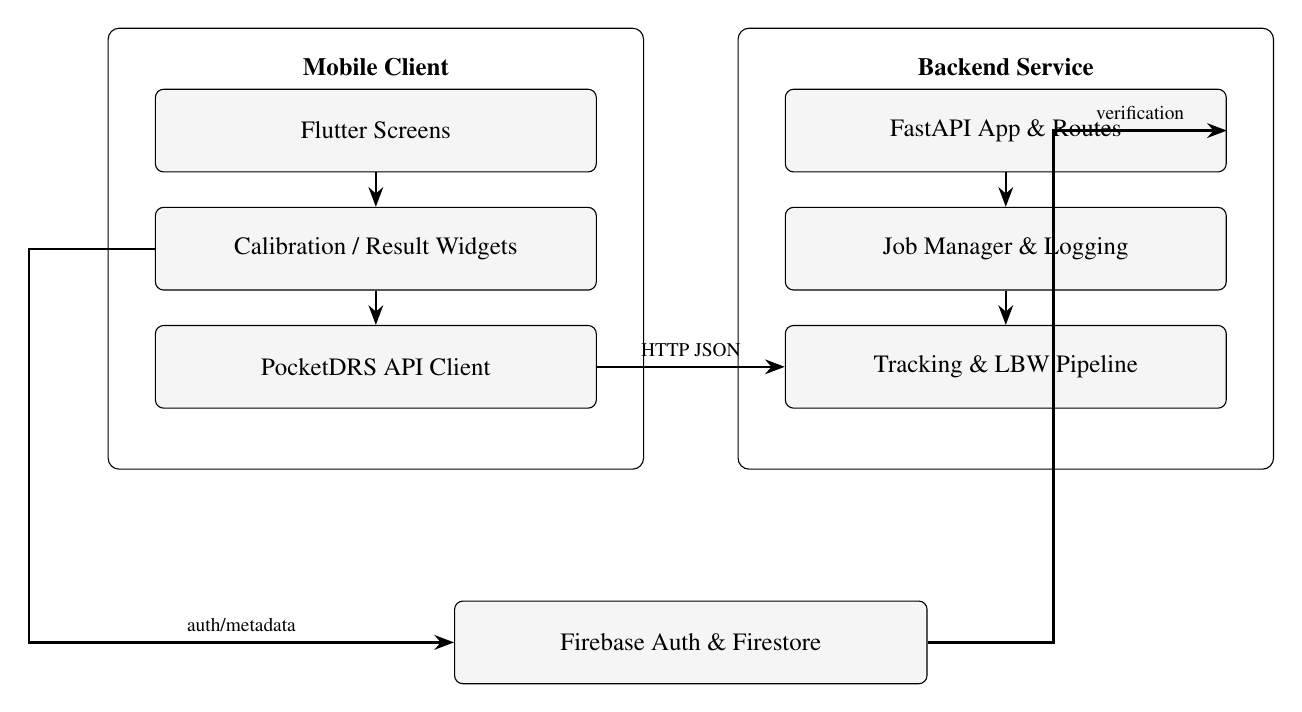
\begin{tikzpicture}[
    pkg/.style={draw, rounded corners=4pt, minimum width=6.8cm, minimum height=5.6cm},
    comp/.style={draw, rounded corners=3pt, minimum width=5.6cm, minimum height=1.05cm, align=center, font=\small, fill=gray!8},
    arrow/.style={-{Stealth[length=2.5mm]}, line width=0.85pt},
    lbl/.style={font=\scriptsize, align=center}
]

\node[pkg] (mobile) at (-4, 0) {};
\node[font=\small\bfseries] at (mobile.north) [yshift=-5mm] {Mobile Client};
\node[comp] (c1) at (-4, 1.5) {Flutter Screens};
\node[comp] (c2) at (-4, 0) {Calibration / Result Widgets};
\node[comp] (c3) at (-4, -1.5) {PocketDRS API Client};

\node[pkg] (backend) at (4, 0) {};
\node[font=\small\bfseries] at (backend.north) [yshift=-5mm] {Backend Service};
\node[comp] (b1) at (4, 1.5) {FastAPI App \& Routes};
\node[comp] (b2) at (4, 0) {Job Manager \& Logging};
\node[comp] (b3) at (4, -1.5) {Tracking \& LBW Pipeline};

\node[comp, minimum width=6.0cm] (firebase) at (0, -5.0) {Firebase Auth \& Firestore};

\draw[arrow] (c1.south) -- (c2.north);
\draw[arrow] (c2.south) -- (c3.north);

\draw[arrow] (b1.south) -- (b2.north);
\draw[arrow] (b2.south) -- (b3.north);

\draw[arrow] (c3.east) -- node[lbl, above] {HTTP JSON} (b3.west |- c3.east);

\draw[arrow] (c2.west) -- ++(-1.6,0) |- node[lbl, above, near end] {auth/metadata} (firebase.west);
\draw[arrow] (firebase.east) -- ++(1.6,0) |- node[lbl, above, near end] {verification} (b1.east);
\end{tikzpicture}
}
\caption{Main software components.}
\label{fig:component}
\end{figure}

\clearpage

\subsubsection{Deployment View}

\begin{figure}[htbp]
\centering
\resizebox{0.96\textwidth}{!}{%
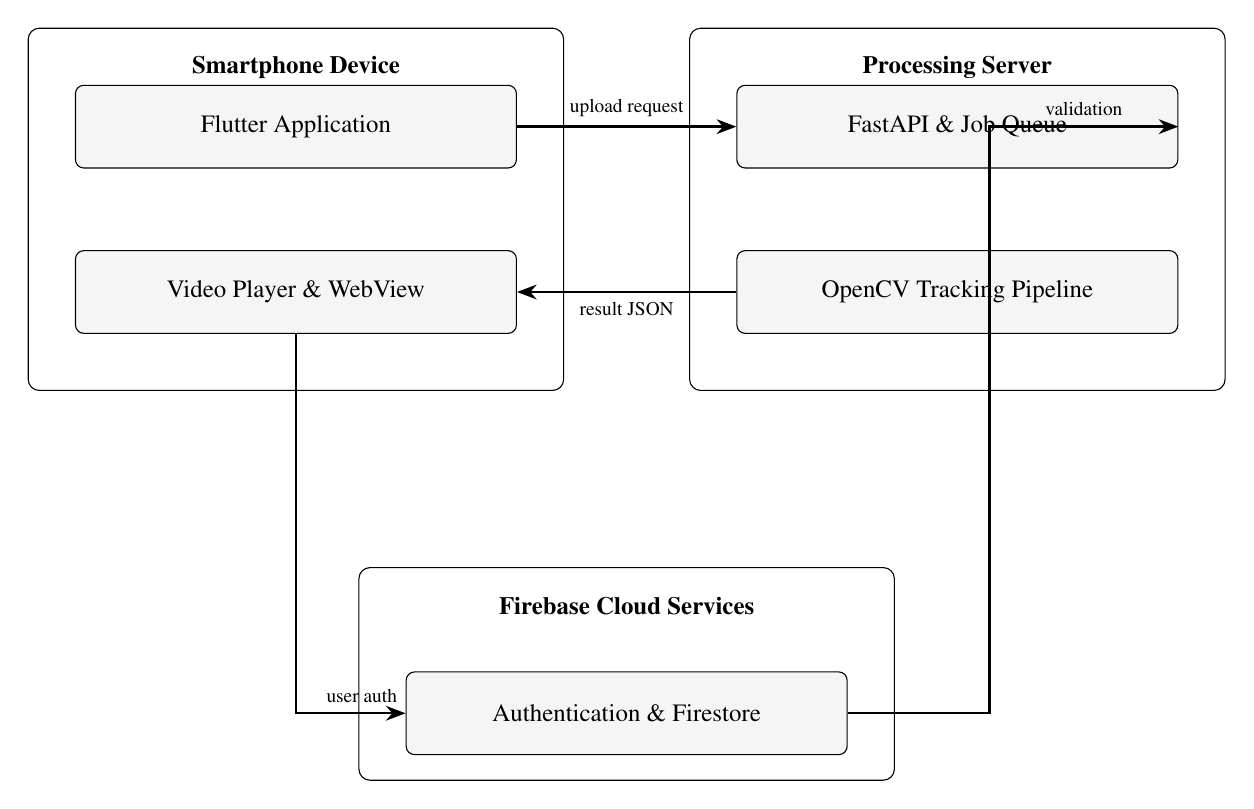
\begin{tikzpicture}[
    nodebox/.style={draw, rounded corners=4pt, minimum width=6.8cm, minimum height=4.6cm, align=center, font=\small},
    inner/.style={draw, rounded corners=3pt, minimum width=5.6cm, minimum height=1.05cm, align=center, font=\small, fill=gray!8},
    arrow/.style={-{Stealth[length=2.5mm]}, line width=0.85pt},
    lbl/.style={font=\scriptsize, align=center}
]

\node[nodebox] (phone) at (-4.2, 0) {};
\node[font=\small\bfseries] at (phone.north) [yshift=-5mm] {Smartphone Device};
\node[inner] (m1) at (-4.2, 1.05) {Flutter Application};
\node[inner] (m2) at (-4.2, -1.05) {Video Player \& WebView};

\node[nodebox] (server) at (4.2, 0) {};
\node[font=\small\bfseries] at (server.north) [yshift=-5mm] {Processing Server};
\node[inner] (s1) at (4.2, 1.05) {FastAPI \& Job Queue};
\node[inner] (s2) at (4.2, -1.05) {OpenCV Tracking Pipeline};

\node[nodebox, minimum height=2.7cm] (cloud) at (0, -5.9) {};
\node[font=\small\bfseries] at (cloud.north) [yshift=-5mm] {Firebase Cloud Services};
\node[inner] (f1) at (0, -6.4) {Authentication \& Firestore};

\draw[arrow] (m1.east) -- node[lbl, above] {upload request} (s1.west);
\draw[arrow] (s2.west) -- node[lbl, below] {result JSON} (m2.east);

\draw[arrow] (m2.south) |- node[lbl, above, pos=0.8] {user auth} (f1.west);
\draw[arrow] (f1.east) -- ++(1.8,0) |- node[lbl, above, near end] {validation} (s1.east);

\end{tikzpicture}
}
\caption{Deployment view of the working system.}
\label{fig:deployment}
\end{figure}

\subsubsection{Current Implementation Status}

The project has progressed beyond initial planning and currently exists as a working prototype. The following summary reflects the present implementation state rather than the long-term vision of the project.

\textbf{Mobile Application.} The Flutter app supports Firebase sign-in, video selection or recording, an interactive pitch calibration step, video trimming, job submission, progress polling, and result display. The calibration workflow collects four pitch corners and stump reference points and validates the geometry before submission.

\textbf{Server and API.} The FastAPI backend accepts authenticated uploads and processes them as background jobs. Each job performs frame decoding, ball tracking, calibration mapping, event estimation, and LBW assessment. The API returns structured JSON including track points, calibration quality, pitch-plane points, bounce and impact indices, decision details, and diagnostic warnings.

\textbf{Ball Tracking Pipeline.} Tracking uses a combined motion-and-colour strategy. A motion detector based on background subtraction is combined with HSV colour filtering so that detections supported by both cues receive higher confidence. A pitch ROI mask derived from the calibration corners restricts the search region and reduces false positives from players, spectators, and background motion.

\textbf{Pitch Calibration and Homography.} The user marks four pitch corners and stump reference points on a reference frame. The backend computes a homography that maps image coordinates to pitch-plane coordinates in meters. When stump points are available, they are used to refine the mapping. A reprojection-based quality score is generated so that low-quality calibration can be flagged.

\textbf{Event Detection and LBW.} Bounce and impact are estimated primarily from the pitch-plane trajectory after calibration. The LBW module then applies rule-based checks for pitching line, impact line, and projected stump contact. The current implementation is a calibrated 2D pitch-plane approximation intended for decision support rather than certified officiating.

\textbf{Visualization Layer.} The result view uses Three.js inside a WebView to display the pitch, stumps, key trajectory points, and decision summary. At the current stage, the visualization is primarily explanatory: the displayed height component is synthesized for presentation, while the core analytical decision is computed from calibrated pitch-plane data.

\textbf{Scope and Limitations.} The current prototype is appropriate for research demonstration, supervised testing, and low-cost review support. It is not ICC-certified, is sensitive to camera placement and lighting, and may fail when the ball is heavily occluded or the calibration input is poor. Full monocular 3D reconstruction remains a future enhancement rather than a completed feature in the current build.

\section{Gantt Chart}

\begin{table}[htbp]
\centering
\caption{Project schedule.}
\label{tab:gantt}
\begin{tabularx}{\textwidth}{@{}Xccccc@{}}
\toprule
\textbf{Task} & \textbf{Dec} & \textbf{Jan} & \textbf{Feb} & \textbf{Mar} & \textbf{Apr} \\
\midrule
Problem identification and literature review & X & X &  &  &  \\
Requirement analysis and system design &  & X & X &  &  \\
Mobile app and backend implementation &  & X & X & X &  \\
Tracking, calibration, and LBW logic &  &  & X & X &  \\
Testing, debugging, and refinement &  &  &  & X & X \\
Documentation and mid/final report updates &  &  &  & X & X \\
\bottomrule
\end{tabularx}
\end{table}

\section{Expected Outcome}

The expected outcome of PocketDRS is a working prototype of a low-cost cricket review-support tool that can:

\begin{enumerate}
    \item Accept a single delivery clip from a phone.
    \item Calibrate the visible pitch using user-selected reference points.
    \item Track the ball through the important part of the delivery.
    \item Map the tracked detections onto pitch-plane coordinates.
    \item Estimate bounce and impact points with diagnostic feedback.
    \item Produce an interpretable LBW decision with a visual explanation.
    \item Demonstrate that a practical DRS-like workflow is possible on a small budget.
\end{enumerate}

In addition, the project is expected to establish a foundation for future work such as stronger ball detectors, more robust calibration, improved prediction models, and true monocular 3D reconstruction. Even in its current form, the system is valuable as a research prototype, a teaching aid, and a demonstration of affordable sports-analytics workflow design.

\section{References}

\begin{thebibliography}{99}

\bibitem{hawkeye2024}
Hawk-Eye Innovations, ``Hawk-Eye: The Technology Behind Sports Officiating,'' 2024. [Online]. Available: \url{https://www.hawkeyeinnovations.com/}

\bibitem{ponglertnapakorn2021}
P. Ponglertnapakorn, T. Shirai, and T. Yamasaki, ``Where Is the Ball: 3D Ball Trajectory Estimation From 2D Monocular Tracking,'' in \textit{Proceedings of the IEEE/CVF Conference on Computer Vision and Pattern Recognition}, 2021.

\bibitem{zhang2000}
Z. Zhang, ``A Flexible New Technique for Camera Calibration,'' \textit{IEEE Transactions on Pattern Analysis and Machine Intelligence}, vol. 22, no. 11, pp. 1330--1334, 2000.

\bibitem{opencv2024}
OpenCV Documentation, ``Camera Calibration and 3D Reconstruction,'' 2024. [Online]. Available: \url{https://docs.opencv.org/}

\bibitem{icc_rules}
International Cricket Council, ``Playing Conditions: Law 36 Leg Before Wicket,'' 2024.

\bibitem{flutter2024}
Google, ``Flutter: Build apps for any screen,'' 2024. [Online]. Available: \url{https://flutter.dev/}

\bibitem{fastapi2024}
S. Ram\'{i}rez, ``FastAPI: Modern, fast web framework for building APIs with Python,'' 2024. [Online]. Available: \url{https://fastapi.tiangolo.com/}

\bibitem{threejs2024}
Three.js Contributors, ``Three.js: JavaScript 3D Library,'' 2024. [Online]. Available: \url{https://threejs.org/}

\end{thebibliography}

\end{document}
